%%%%% Literature Review %%%%%
\section{Literature Review} 
In the last two decades, significant progress in electronic and computer technologies has led to remarkable 
growth in the field of manipulator robotics. Manipulators developed by various institutions have been integrated 
into the industrial sector to autonomously or semi-autonomously perform repetitive tasks. Simultaneously, 
manipulators are utilized for tasks with stringent precision requirements to minimize errors. Additionally, 
essential tasks are undertaken by manipulators to substitute for humans in challenging environments. 
%%%%% Manipulator Utilization in Biology Field %%%%%
\subsection{Manipulators in Biomedical Applications}
With a growing emphasis on the field of biology, manipulators have also been introduced to assist. 
In the field of medicine, manipulators have been utilized since the end of the last century 
\cite{AESOP,ZEUS,ZEUS_example1,ZEUS_example2,ZEUS_example3}. At the beginning of the 21st century, a novel 
robotic system, da Vinci robotic surgery system, was designed to facilitate more intricate surgical procedures 
\cite{da_Vinci}. Moreover, manipulators can be leveraged in the field of biological physics as a viable approach 
for biological experiments. In the HIFU system developed by An et al., the SCARA (self compliant automatic robot 
assembly) robot was employed as manipulator, incorporating an ultrasound probe to scan 
biological tissues \cite{HIFU2017}. The robotic system FUSBOTs (Focal Ultrasound Surgery RoBOTs) was proposed 
and upgraded to accomplish more precise targeted treatment with multiple DoF (Degrees of Freedom) manipulators 
\cite{FUSBOT,FUSBOT_example1,FUSBOT_example2}. Despite the various utilization of manipulator platforms 
designed for accommodating ultrasonic transducers \cite{6DOF_HIFU,6DOF_HIFU_comp,6DOF_HIFU_ABB}, 
certain limitations persist. A comparison between different types of manipulators is necessary in the 
selection of appropriate type manipulator for integrating ultrasonic transducer. 
%%%%% Manipulator Types %%%%%
\subsection{Types of Manipulator }
From the perspective of geometry, rigid-body manipulators can be categorized into two main types: parallel 
mechanisms and serial links \cite{MECH0089book}. The control of parallel mechanisms is relatively complex. 
Meanwhile, serial link manipulators can be further divided into five types: Cartesian (PPP), articulated (RRR), 
cylindrical (RPP), spherical (RRP), and SCARA (RRP). Additionally, with the advancement of robotics technology, 
two other types of manipulators, namely biomimetic and anthropomorphic, have demonstrated their advantages 
\cite{manipulators_types1,manipulators_types2}.
The comparative analysis will be conducted to highlight the distinctive features of different manipulators 
presented in Table \ref{tab:different_types_manipulators}, leading to the identification of the most suitable 
type for specific applications.
\begin{center}
    \small
    \begin{longtable}{l c c l l}
    \caption{The Characteristics of Different Manipulators.} 
    \label{tab:different_types_manipulators} \\
    \hline \multicolumn{1}{c}{\textbf{Manipulators}} & 
    \multicolumn{1}{c}{\textbf{Types}} & 
    \multicolumn{1}{c}{\textbf{DoF}} & 
    \multicolumn{1}{c}{\textbf{Features}} & 
    \multicolumn{1}{c}{\textbf{Applications}} \\ \hline 
    \endfirsthead
    \multicolumn{5}{c}%
    {{\bfseries \tablename\ \thetable{} -- continued from previous page}} \\
    \hline \multicolumn{1}{c}{\textbf{Manipulators}} & 
    \multicolumn{1}{c}{\textbf{Types}} & 
    \multicolumn{1}{c}{\textbf{DoF}} & 
    \multicolumn{1}{c}{\textbf{Features}} & 
    \multicolumn{1}{c}{\textbf{Applications}} \\ \hline 
    \endhead
    \hline \multicolumn{5}{|r|}{{Continued on next page}} \\ \hline
    \endfoot
    \hline \hline
    \endlastfoot
    % table context
    \multirow{2}{25mm}{Stewart Platform \cite{stewart}}& 
    \multirow{2}{*}{\parbox{15mm}{Series-Parallel}} & 6 & 
    series-parallel duality, &
    flight simulation \cite{flight_simulation}. \\
    & & & mature kinematics & robocrane \cite{RoboCrane}\\ 
    & & & algorithm. & \\ 
    Cartesian & PPP & 3 &
    technological maturity, &
    3D-Printing framework \cite{PPP_3Dprint} \\
    & & & low complexity, cost-& warehousing \& hoisting \cite{PPP_warehouse}\\ 
    & & & effective, high payload. & agricultural machinery \cite{PPP_agriculture}\\ 
    Articulated \cite{RRR_feature}& RRR & 6 & 
    factory automation,   &
    milling operations \cite{RRR_application1} \\
    & & & programmable, high & material handling \cite{RRR_application2} \\ 
    & & & precision and payload.& \\ 
    Cylindrical \cite{SCARA_review}& RPP & 3 & 
    good precision, limited  &
    assembling industries \cite{RPP_application} \\
    & & & workspace. & \\
    Spherical \cite{RRP_feature}& RRP & 3 & 
    \multirow{3}{*}{\parbox{40mm}{collision avoidance, low precision, long reach, light weight.}} &
    low-precision semi- \\
    & & & & automated tasks \cite{RRR_application1,RRR_application2}\\
    & & & & \\
    SCARA \cite{SCARA_review}& RRP & 3 & 
    high accuracy and fast  &
    surgical applications \cite{SCARA_application1}\\
    & & & operation. & medical rehabilitation \cite{SCARA_application2}\\
    \multirow{2}{25mm}{Continuum/ Soft \cite{soft_review1,soft_review2}} & Biomimetic & $\infty$ & 
    ability to handle  & 
    tendon driven \cite{tenden_driven_application1, tenden_driven_application2,tenden_driven_application3}\\
    & & & fatigue objects, & fibre-reinforced \cite{fiber_application1,fiber_application2}\\
    & & & environmental & fluid-elastic drive \cite{fluid_application1,fluid_application2,fluid_application3}\\
    & & & adaptability. & bionics materials \cite{SMA,dielectric_high-elastic_polymers,IPMC}\\
    Humanoid & anthropo- & 7 & high efficiency, & humanoid robots driven \\
    & morphic& & flexibility.& by pneumatic artificial\\ 
    & & & & muscles \cite{humanoid_7dof}\\ \hline
    \end{longtable}
\end{center}
\vspace{-10mm}
\noindent The distinctive structure of the continuum manipulator imparts to the system with theoretically 
infinite DoF. The characteristic enables the continuum manipulator to navigate through confined spaces 
or manipulate objects along specific trajectories within the workspace \cite{CR_medical_application,
soft_review1,soft_review2}. Simultaneously, the continuum robotic
manipulator demonstrates suboptimal performance in the context of payload, making it challenging to meet 
the payload capacities commonly observed in industrial robotic systems. Nevertheless, within the realm 
of biomedical applications, the emphasis shifts towards precision and operability for manipulators. In this 
report, the manipulator platform integrated with the ultrasonic transducer module necessitates a design. 
The selection of the continuum manipulator was predicated upon its outstanding flexibility and the 
lightweight attributes of the ultrasonic transducer module. An appropriate type of continuum robot 
will be selected to serve as the centrepiece for the manipulator platform.
%%%%% Continuum Robots Types %%%%%
\subsection{Types of Continuum Robots}
Nowadays, a variety of continuum robots exist, each exhibiting unique structures and functions. They serve in different fields 
such as medicine, construction, and exploration. In this section, some of the most popular continuum robots will be introduced, 
providing basic insights into their structures as well as discussing their merits and drawbacks. \\
\vspace{-10mm}
\subsubsection{Tendon-Driven Robots}
The arm of the Tendon-Driven robot consists of a backbone, several tendons and disks. The backbone defines the structure and 
posture of the entire robot arm, while disks define the diameter and divide the robot arm into segments, and tendons are 
stretched to create deformation and movements of different directions for the robot arm. \\
Figure \ref{fig:3tendon_1segment_CR} shows only the simplest tenon-driven robots. In practical applications, there 
may be more than one backbone, and the disks are not necessarily parallel. \\
Compared with other continuum robots, one of the most significant advantages of tendon-driven robots is their flexibility. 
This advantage makes it more effective in performing tasks in complex and restrictive Spaces. In addition, due to the simple 
components needed to construct the robot, it is easier to meet lightweight design specifications. Moreover, like the 
concentric-tube continuum robots, tendon-driven continuum robots can be built and designed on a small scale with diameters of 
below 10 mm \cite{amanov2021tendon}. \\
However, due to its simple actuating principle, more complex algorithms are needed to control it more accurately. Also, the 
tendon-driven robots actuate by pulling the tendon, which makes the friction between the tendon and other components inevitable, 
which will accelerate the wearing speed of the tendon-driven robots.
\begin{figure}[H] % figure
    \centering
    \captionsetup{labelsep=colon}
    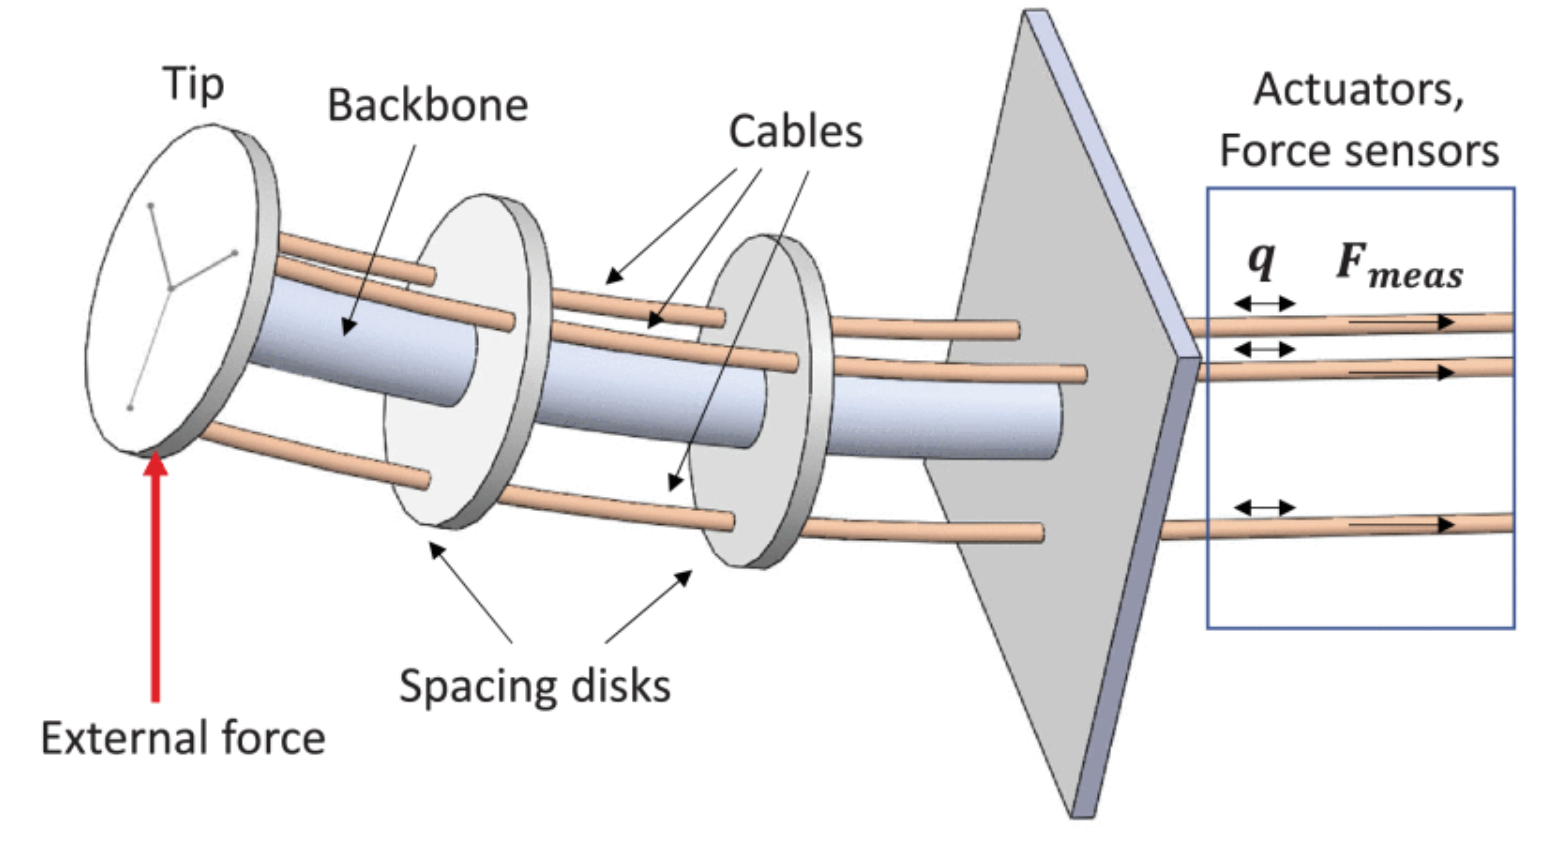
\includegraphics[width=.7\textwidth]{Image/LR/3tendon_1segment_CR.PNG} 
    \caption[A three-tendons continuum robot with one segment]
    {\centering \textbf{A three-tendons continuum robot with one segment} \cite{3tendon_1segment_CR}.}
    \label{fig:3tendon_1segment_CR}
\end{figure}
\subsubsection{Fishbone Robots}
Fishbone robots are inspired by fish bones. It is consists of several "fishbone moduless", which are 
composed of a number of rigid cross-shaped plates, and a flexible elastic plate backbone embedded in the middle, 
forming a rigid-soft coupling structure\cite{fishboneCR}. 
\begin{figure}[H] % figure
    \centering 
    \captionsetup{labelsep=colon}
    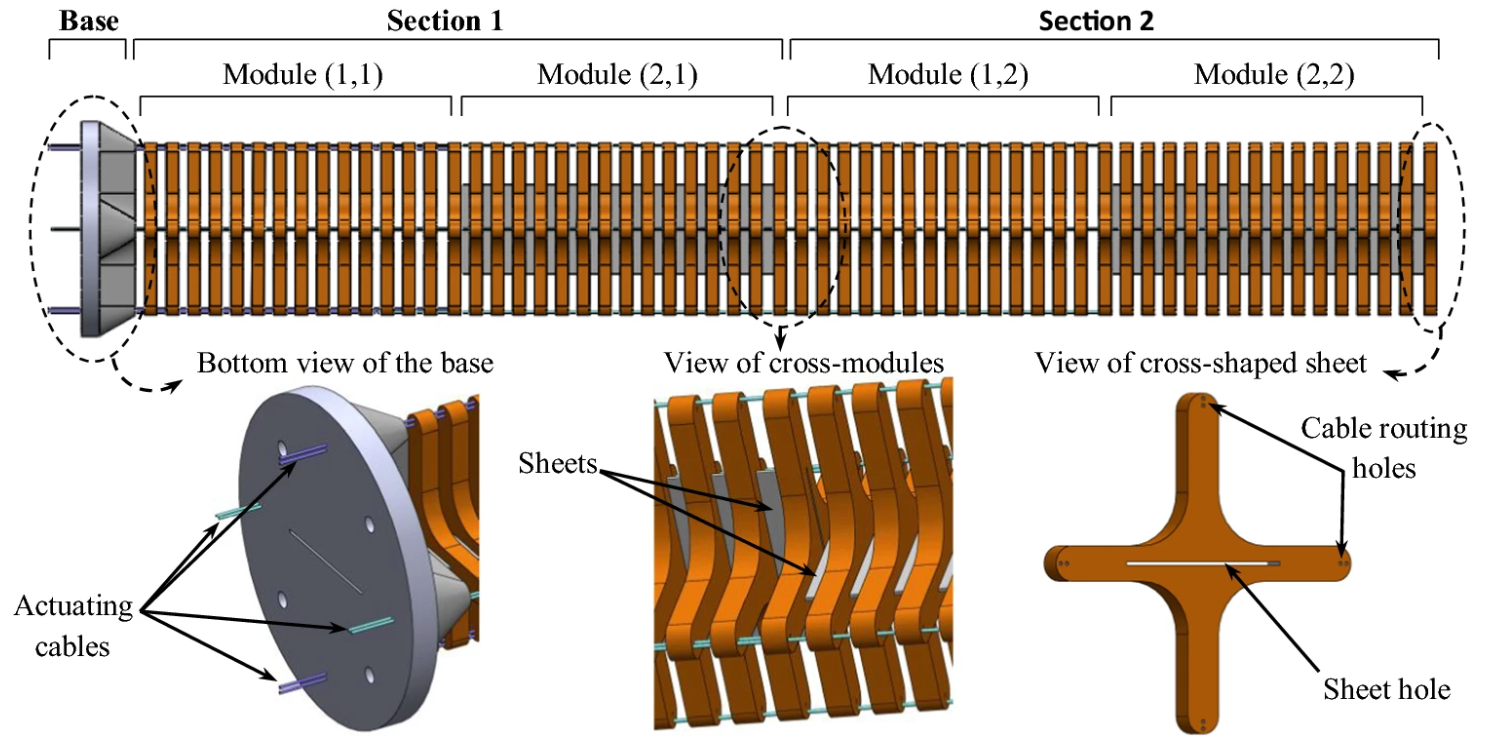
\includegraphics[width=.9\textwidth]{Image/LR/fishbone_CR_amouri2023bio.PNG} 
    \caption[The cable-driven fishbone continuum robot]
    {\centering \textbf{The cable-driven fishbone continuum robot with cable arrangement} \cite{amouri2023bio}.}
    \label{fig:fishboneCR_2023bio}
\end{figure}
\noindent According to Figure \ref{fig:fishboneCR_2023bio}, when the different modules are connected, the backbones of the bionic 
fishbone modules are perpendicular to each other, and finally form a complete main frame of the fishbone robot. Like the 
tendon-driven robot, the fishbone robot is also controlled by cable, but it is worth noting that each module is controlled 
by two separate cables. This means that for a fishbone robot composed of n fishbone modules, there are a total of 2n cables 
controlling the motionof the whole robot. In addition, the planes formed by the two ropes that control each module are 
perpendicular to each other, so that each section rotates along a plane perpendicular to each other. \\
The Figure \ref{fig:fishboneCR_2023bio} shows that because of the numbers of rigid cross-shaped sheets formed a large diameter 
frame, the structural stability of this kind of robot is very strong. Also, each fishbone unit can provide one DoF, making it 
easy to reach a very high total DoF. However, due to the multiple-curves deformation trajectory, the fishbone robots are not 
suitable for situations where strict trajectory is required\cite{fishboneCR}. 
\subsubsection{Concentric Tube Continuum Robots}
The concentric tube robots, shaped like retractable walking sticks, consist of many tubes with decreasing diameters. Each tube is 
nested on top of the previous wider tube.  \\
The concentric robots are made of two parts: tubes and coaxial actuation units. The tubes are the main structural element of 
this robot and act as the backbone. The coaxial actuation unit consists of two motors which are responsible for rotation and 
translation movement respectively. Each tube is actuated by an independent coaxial actuation unit. 
\begin{figure}[H] % figure
    \centering 
    \captionsetup{labelsep=colon}
    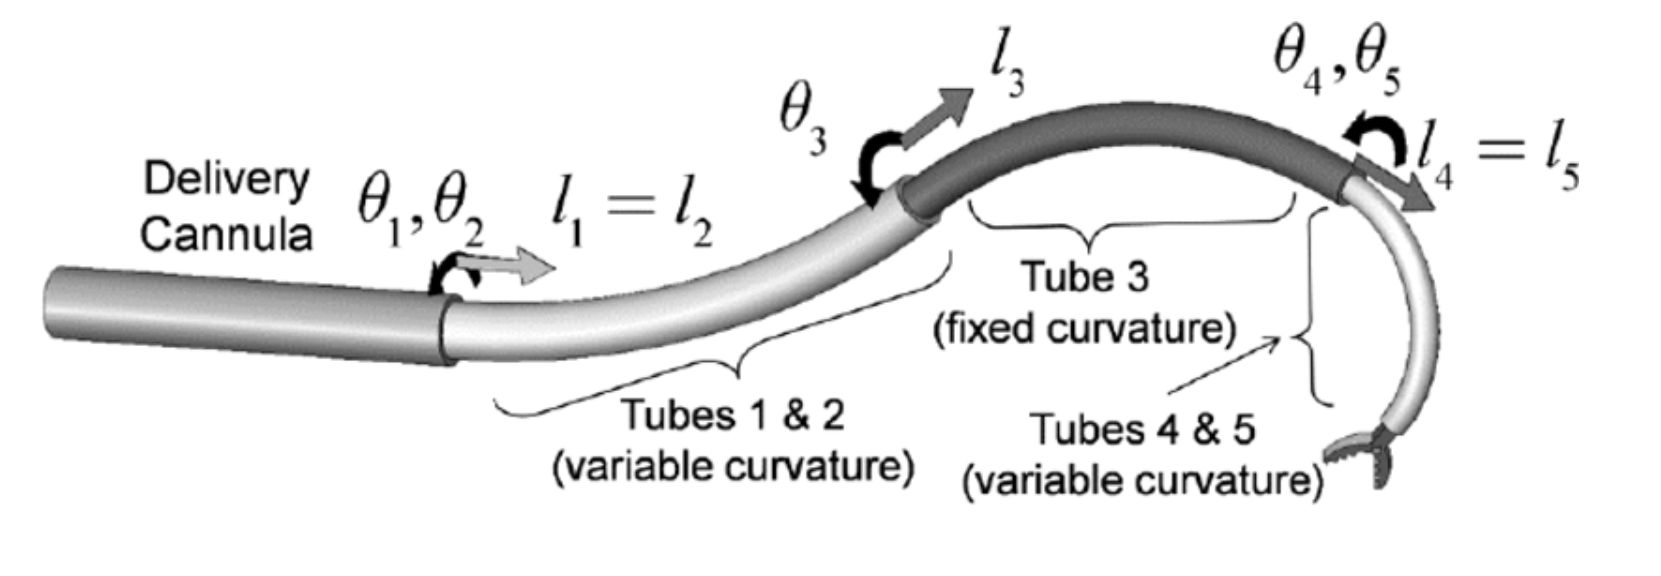
\includegraphics[width=.8\textwidth]{Image/LR/concentric_tube_CR.PNG} 
    \caption[An example concentric tube continuum robot]
    {\centering \textbf{An example concentric tube continuum robot} \cite{CTCR_example}.}
    \label{fig:CTCR_example}
\end{figure}
\noindent The most significant advantage of this kind of robots is that of all the continuum robots, concentric tube robots have the 
smallest possible outer diameter and are best suited to work in confined and narrow Spaces. Therefore, it is the ideal choice 
for surgical operations. \\
Their disadvantages, on the other hand, are also very evident. Since each tube requires an independent actuation unit, the 
overall length of the robot cannot be very long, because longer lengths will lead to more tubes, and will lead to more tip 
position errors.

% change to new page
\newpage